% Created by tikzDevice version 0.12.6 on 2026-05-17 18:10:45
% !TEX encoding = UTF-8 Unicode
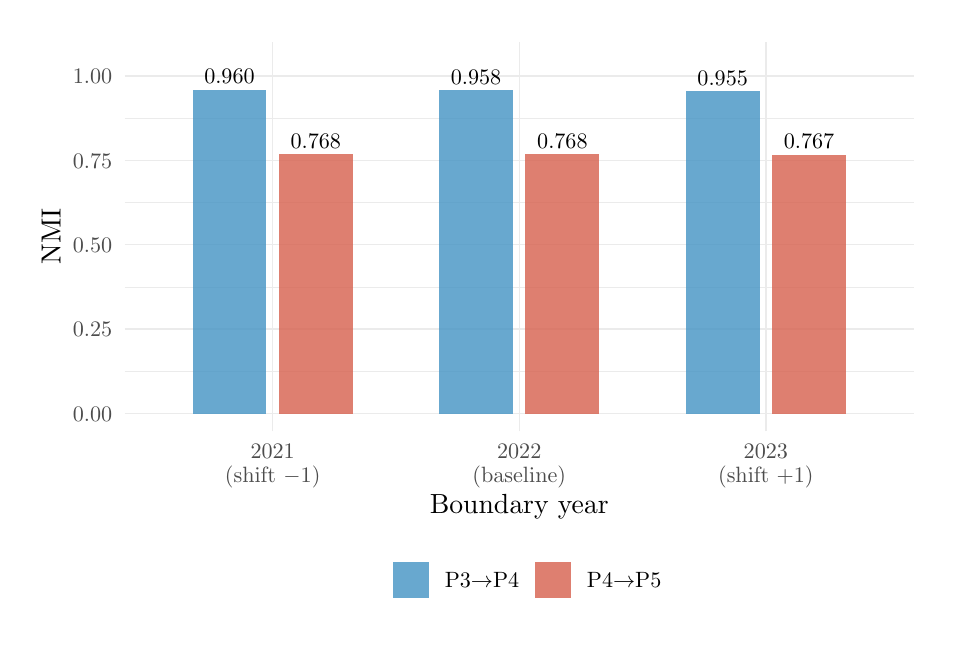
\begin{tikzpicture}[x=1pt,y=1pt]
\definecolor{fillColor}{RGB}{255,255,255}
\path[use as bounding box,fill=fillColor,fill opacity=0.00] (0,0) rectangle (325.21,216.81);
\begin{scope}
\path[clip] (  0.00,  0.00) rectangle (325.21,216.81);
\definecolor{fillColor}{RGB}{255,255,255}

\path[fill=fillColor] ( -0.00,  0.00) rectangle (325.21,216.81);
\end{scope}
\begin{scope}
\path[clip] ( 35.05, 70.99) rectangle (320.21,211.81);
\definecolor{drawColor}{gray}{0.92}

\path[draw=drawColor,line width= 0.3pt,line join=round] ( 35.05, 92.63) --
	(320.21, 92.63);

\path[draw=drawColor,line width= 0.3pt,line join=round] ( 35.05,123.11) --
	(320.21,123.11);

\path[draw=drawColor,line width= 0.3pt,line join=round] ( 35.05,153.59) --
	(320.21,153.59);

\path[draw=drawColor,line width= 0.3pt,line join=round] ( 35.05,184.07) --
	(320.21,184.07);

\path[draw=drawColor,line width= 0.5pt,line join=round] ( 35.05, 77.39) --
	(320.21, 77.39);

\path[draw=drawColor,line width= 0.5pt,line join=round] ( 35.05,107.87) --
	(320.21,107.87);

\path[draw=drawColor,line width= 0.5pt,line join=round] ( 35.05,138.35) --
	(320.21,138.35);

\path[draw=drawColor,line width= 0.5pt,line join=round] ( 35.05,168.83) --
	(320.21,168.83);

\path[draw=drawColor,line width= 0.5pt,line join=round] ( 35.05,199.31) --
	(320.21,199.31);

\path[draw=drawColor,line width= 0.5pt,line join=round] ( 88.52, 70.99) --
	( 88.52,211.81);

\path[draw=drawColor,line width= 0.5pt,line join=round] (177.63, 70.99) --
	(177.63,211.81);

\path[draw=drawColor,line width= 0.5pt,line join=round] (266.75, 70.99) --
	(266.75,211.81);
\definecolor{fillColor}{RGB}{67,147,195}

\path[fill=fillColor,fill opacity=0.80] ( 59.56, 77.39) rectangle ( 86.29,194.44);

\path[fill=fillColor,fill opacity=0.80] (148.67, 77.39) rectangle (175.40,194.19);

\path[fill=fillColor,fill opacity=0.80] (237.78, 77.39) rectangle (264.52,193.83);
\definecolor{fillColor}{RGB}{214,96,77}

\path[fill=fillColor,fill opacity=0.80] ( 90.75, 77.39) rectangle (117.48,171.03);

\path[fill=fillColor,fill opacity=0.80] (179.86, 77.39) rectangle (206.59,171.03);

\path[fill=fillColor,fill opacity=0.80] (268.97, 77.39) rectangle (295.71,170.91);
\definecolor{drawColor}{RGB}{0,0,0}

\node[text=drawColor,anchor=base,inner sep=0pt, outer sep=0pt, scale=  0.80] at ( 72.92,196.63) {0.960};

\node[text=drawColor,anchor=base,inner sep=0pt, outer sep=0pt, scale=  0.80] at (162.04,196.39) {0.958};

\node[text=drawColor,anchor=base,inner sep=0pt, outer sep=0pt, scale=  0.80] at (251.15,196.02) {0.955};

\node[text=drawColor,anchor=base,inner sep=0pt, outer sep=0pt, scale=  0.80] at (104.11,173.22) {0.768};

\node[text=drawColor,anchor=base,inner sep=0pt, outer sep=0pt, scale=  0.80] at (193.23,173.22) {0.768};

\node[text=drawColor,anchor=base,inner sep=0pt, outer sep=0pt, scale=  0.80] at (282.34,173.10) {0.767};
\end{scope}
\begin{scope}
\path[clip] (  0.00,  0.00) rectangle (325.21,216.81);
\definecolor{drawColor}{gray}{0.30}

\node[text=drawColor,anchor=base east,inner sep=0pt, outer sep=0pt, scale=  0.80] at ( 30.55, 74.64) {0.00};

\node[text=drawColor,anchor=base east,inner sep=0pt, outer sep=0pt, scale=  0.80] at ( 30.55,105.12) {0.25};

\node[text=drawColor,anchor=base east,inner sep=0pt, outer sep=0pt, scale=  0.80] at ( 30.55,135.60) {0.50};

\node[text=drawColor,anchor=base east,inner sep=0pt, outer sep=0pt, scale=  0.80] at ( 30.55,166.08) {0.75};

\node[text=drawColor,anchor=base east,inner sep=0pt, outer sep=0pt, scale=  0.80] at ( 30.55,196.56) {1.00};
\end{scope}
\begin{scope}
\path[clip] (  0.00,  0.00) rectangle (325.21,216.81);
\definecolor{drawColor}{gray}{0.30}

\node[text=drawColor,anchor=base,inner sep=0pt, outer sep=0pt, scale=  0.80] at ( 88.52, 60.98) {2021};

\node[text=drawColor,anchor=base,inner sep=0pt, outer sep=0pt, scale=  0.80] at ( 88.52, 52.34) {(shift $-1$)};

\node[text=drawColor,anchor=base,inner sep=0pt, outer sep=0pt, scale=  0.80] at (177.63, 60.98) {2022};

\node[text=drawColor,anchor=base,inner sep=0pt, outer sep=0pt, scale=  0.80] at (177.63, 52.34) {(baseline)};

\node[text=drawColor,anchor=base,inner sep=0pt, outer sep=0pt, scale=  0.80] at (266.75, 60.98) {2023};

\node[text=drawColor,anchor=base,inner sep=0pt, outer sep=0pt, scale=  0.80] at (266.75, 52.34) {(shift $+1$)};
\end{scope}
\begin{scope}
\path[clip] (  0.00,  0.00) rectangle (325.21,216.81);
\definecolor{drawColor}{RGB}{0,0,0}

\node[text=drawColor,anchor=base,inner sep=0pt, outer sep=0pt, scale=  1.00] at (177.63, 41.40) {Boundary year};
\end{scope}
\begin{scope}
\path[clip] (  0.00,  0.00) rectangle (325.21,216.81);
\definecolor{drawColor}{RGB}{0,0,0}

\node[text=drawColor,rotate= 90.00,anchor=base,inner sep=0pt, outer sep=0pt, scale=  1.00] at ( 11.89,141.40) {NMI};
\end{scope}
\begin{scope}
\path[clip] (  0.00,  0.00) rectangle (325.21,216.81);
\definecolor{fillColor}{RGB}{67,147,195}

\path[fill=fillColor,fill opacity=0.80] (131.94, 10.65) rectangle (145.10, 23.81);
\end{scope}
\begin{scope}
\path[clip] (  0.00,  0.00) rectangle (325.21,216.81);
\definecolor{fillColor}{RGB}{214,96,77}

\path[fill=fillColor,fill opacity=0.80] (183.28, 10.65) rectangle (196.44, 23.81);
\end{scope}
\begin{scope}
\path[clip] (  0.00,  0.00) rectangle (325.21,216.81);
\definecolor{drawColor}{RGB}{0,0,0}

\node[text=drawColor,anchor=base west,inner sep=0pt, outer sep=0pt, scale=  0.80] at (150.75, 14.47) {P3$\to$P4};
\end{scope}
\begin{scope}
\path[clip] (  0.00,  0.00) rectangle (325.21,216.81);
\definecolor{drawColor}{RGB}{0,0,0}

\node[text=drawColor,anchor=base west,inner sep=0pt, outer sep=0pt, scale=  0.80] at (202.09, 14.47) {P4$\to$P5};
\end{scope}
\end{tikzpicture}
